% Figures for "Non-Branching Is Not Enough".
% Included from main.tex. Kept separate so a figure can be rebuilt and
% inspected without recompiling the whole paper.
%
% Deliberately monochrome: these are structural diagrams, and the distinctions
% that matter (identical vs differing, admitted vs rejected) are carried by
% shape and label, not by colour. They survive greyscale printing.

% ---------------------------------------------------------------- Figure 1
% The gap, shown on real data: identical control flow, differing output.
\newcommand{\figSequenceVsValue}{%
\begin{figure}[t]
\centering
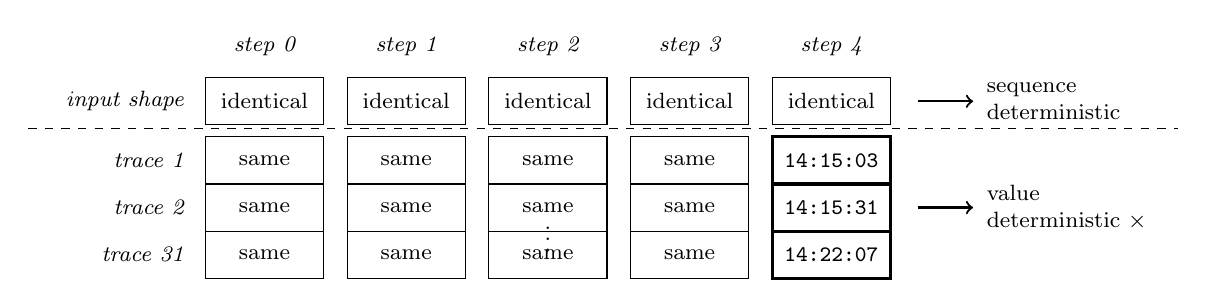
\begin{tikzpicture}[
  font=\footnotesize,
  cell/.style={draw, minimum width=15mm, minimum height=6mm, inner sep=1pt},
  same/.style={cell},
  differs/.style={cell, very thick},
  lbl/.style={font=\footnotesize\itshape},
]

% column headers
\node[lbl] at (0,  0.9) {step 0};
\node[lbl] at (1.8,0.9) {step 1};
\node[lbl] at (3.6,0.9) {step 2};
\node[lbl] at (5.4,0.9) {step 3};
\node[lbl] at (7.2,0.9) {step 4};

% input-shape row
\node[lbl, anchor=east] at (-0.9, 0.2) {input shape};
\foreach \x in {0, 1.8, 3.6, 5.4, 7.2}
  \node[same] at (\x, 0.2) {identical};

% output rows, one per trace
\foreach \y/\name in {-0.55/trace 1, -1.15/trace 2, -1.75/trace 31} {
  \node[lbl, anchor=east] at (-0.9, \y) {\name};
  \foreach \x in {0, 1.8, 3.6, 5.4}
    \node[same] at (\x, \y) {same};
}
\node[differs] at (7.2, -0.55) {\ttfamily 14:15:03};
\node[differs] at (7.2, -1.15) {\ttfamily 14:15:31};
\node[differs] at (7.2, -1.75) {\ttfamily 14:22:07};

% vertical ellipsis between trace 2 and trace 31
\node at (3.6, -1.45) {$\vdots$};

% verdicts
\draw[->, thick] (8.3, 0.2) -- (9.0, 0.2);
\node[anchor=west, align=left] at (9.05, 0.2)
  {sequence\\deterministic \checkmark};
\draw[->, thick] (8.3, -1.15) -- (9.0, -1.15);
\node[anchor=west, align=left] at (9.05, -1.15)
  {value\\deterministic $\times$};

\draw[dashed] (-3.0, -0.15) -- (11.6, -0.15);
\end{tikzpicture}
\caption{The gap, from the corpus. All five steps of the governance workflow
share an identical input shape at every position across 31 traces, so the
published control-flow criterion promotes the workflow. Step~4 appends to an
audit log and returns a different timestamp on every run for byte-identical
input. Promoting it yields an artifact that replays a stale value silently.}
\label{fig:gap}
\end{figure}
}

% ---------------------------------------------------------------- Figure 2
% Two gates and the set each admits. The shaded difference is the finding.
\newcommand{\figTwoGates}{%
\begin{figure}[t]
\centering
\begin{tikzpicture}[
  font=\footnotesize,
  box/.style={draw, rounded corners=2pt, minimum width=30mm,
              minimum height=8mm, align=center},
  gate/.style={draw, diamond, aspect=2.2, inner sep=1pt, align=center,
               minimum width=26mm},
  % NB: not named "out" - that collides with TikZ's built-in path key.
  result/.style={draw, minimum width=26mm, minimum height=7mm, align=center},
]

\node[box] (cand) at (0,0) {candidate workflow\\\itshape $m \geq 10$ traces};

\node[gate] (cf) at (0,-1.8) {control flow\\stable?};
\node[gate] (pu) at (0,-4.0) {outputs\\reproduce?};

\node[result] (rej1) at (5.2,-1.8) {reject\\\itshape keep observing};
\node[result, very thick] (rej2) at (5.2,-4.0)
  {\textbf{reject}\\\itshape this work};
\node[result] (seal) at (0,-5.9) {promote / seal};

\draw[->] (cand) -- (cf);
\draw[->] (cf) -- node[right, pos=0.45] {yes} (pu);
\draw[->] (cf) -- node[above, pos=0.45] {no} (rej1);
\draw[->] (pu) -- node[right, pos=0.45] {yes} (seal);
\draw[->] (pu) -- node[above, pos=0.45] {no} (rej2);

% what the published criterion does
\draw[dashed, very thick, rounded corners=3pt]
  (-2.6,-2.55) rectangle (2.6,-1.05);
\node[anchor=west, font=\footnotesize\itshape] at (-2.55,-2.8)
  {published criterion stops here};

\node[anchor=west, align=left, font=\footnotesize] at (7.0,-4.0)
  {1 of 16 observable steps\\
   in our corpus reaches\\
   this box (\S\ref{sec:results})};

\end{tikzpicture}
\caption{Two gates. Published promotion criteria test the first. A step that
passes control-flow stability and fails output reproducibility is promoted by
those criteria and rejected here; the bold box is the difference this paper
measures.}
\label{fig:gates}
\end{figure}
}

% ---------------------------------------------------------------- Figure 3
% Oracle vs detector: what each can and cannot see.
\newcommand{\figOracleDetector}{%
\begin{figure}[t]
\centering
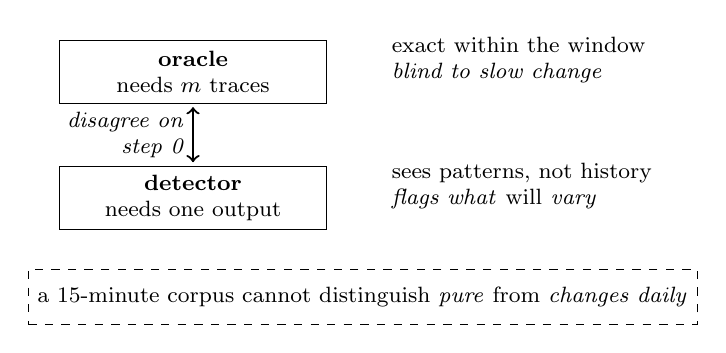
\begin{tikzpicture}[
  font=\footnotesize,
  band/.style={draw, minimum height=8mm, align=center, inner sep=3pt},
]

\node[band, minimum width=34mm] (oracle) at (0,0)
  {\textbf{oracle}\\needs $m$ traces};
\node[band, minimum width=34mm] (det) at (0,-1.6)
  {\textbf{detector}\\needs one output};

\node[align=left, anchor=west, font=\footnotesize] at (2.4, 0.15)
  {exact within the window\\
   \itshape blind to slow change};
\node[align=left, anchor=west, font=\footnotesize] at (2.4, -1.45)
  {sees patterns, not history\\
   \itshape flags what \emph{will} vary};

\draw[<->, thick] (0,-0.45) -- (0,-1.15)
  node[midway, left, font=\footnotesize\itshape, align=right]
  {disagree on\\step 0};

\node[draw, dashed, minimum width=78mm, minimum height=7mm, anchor=north west,
      align=center, font=\footnotesize] at (-2.1,-2.5)
  {a 15-minute corpus cannot distinguish
   \emph{pure} from \emph{changes daily}};

\end{tikzpicture}
\caption{The two purity signals are complementary rather than ranked. The
oracle is exact over observed traces and blind beyond them; the detector
encodes knowledge the observation window cannot supply. Our single false
positive (\S\ref{sec:fp}) is this disagreement, not an error.}
\label{fig:oracle}
\end{figure}
}
